% ============================================================
% Materials and Methods section -- meant to be \input{} or \include{}'d
% from a main manuscript file, not compiled standalone. Same
% bibliography/style requirements as introduction.tex (see that file's
% header comment). Also requires \usepackage{url} (or hyperref, which
% loads it) for the \url{} dataset-availability links in Section 3.1, and
% \usepackage{graphicx} for the \includegraphics{} figures in Section 3.3
% (figures/encoding_diagram.pdf from figures/make_encoding_diagram.py, and
% figures/transfer_functions.pdf from
% figures/make_transfer_function_diagram.py -- rerun the relevant script
% if either description ever changes, rather than hand-editing the PDF).
% The transfer-function plot's closed forms were derived from the real
% project code and cross-checked against it by Monte Carlo simulation
% (asserted in the script itself) before being plotted as smooth curves;
% this process surfaced that transfer.py::v_shaped's docstring ("flips
% the previous bit with probability V(x)") does not match its own
% measured behavior (flip probability is actually 1-V(x), peaking at
% x=0) -- flagged here for awareness, not silently resolved either way;
% verify against Hashemi et al.'s literal Eq. 6-7 before treating either
% the docstring or the code as authoritative.
%
% CITATION STATUS: every \cite{...} below resolves to a real, verified
% entry in references.bib (Little:2008, Naranjo:2016, Cheng:2015, and the
% 5 baseline source papers, all already used and verified elsewhere in
% this manuscript).
%
% DATA STATUS: all dataset statistics (sample sizes, subject counts,
% feature counts, class balance) were read directly from
% `src/data_loader.py` and a live run of `python -m src.data_loader`, not
% recalled from memory or from the source papers' own stated counts. Two
% discrepancies against externally-quoted figures were found and are
% documented in the note in Section \ref{sec:3.1}: the Oxford subject
% count (32, vs. the commonly quoted "31 subjects") and the UCI
% repository listing's structured "197 instances" metadata field (vs.
% 195, which matches both the actual distributed data file and that same
% listing's own descriptive prose) -- confirmed by fetching the live UCI
% page at https://archive.ics.uci.edu/dataset/174/parkinsons, not assumed.
%
% ENCODING STATUS (as of the latest revision): EOACSO (and its ablation
% variants) uses the project's own multi-classifier soft-voting ensemble
% (`decode_bits`); the 7 reproduced baselines always decode top-1
% (`decode_bits_top1`). This has been a genuinely unstable design
% decision across the project's history -- if asked to touch this file
% again, RE-CONFIRM the current default in `src/optimizers/base.py` and
% `src/experiments/run_comparison.py`/`run_ablation.py` before assuming
% this description is still accurate.
% ============================================================

\section{Materials and Methods}
\label{sec:3}

\subsection{Datasets and Study Population}
\label{sec:3.1}

Two public, retrospective, previously collected acoustic datasets are
used; no new data were collected for this study.

\textbf{Oxford Parkinson's Disease Voice Dataset} \cite{Little:2008},
publicly available from the UCI Machine Learning Repository
(\url{https://archive.ics.uci.edu/dataset/174/parkinsons},
\url{https://doi.org/10.24432/C59C74}), comprises 195 sustained phonation
(vowel /a/) recordings from 32 subjects, drawn from the \texttt{name}
field's subject code (\emph{not} the 31 patients reported in the
dataset's originating clinical study -- see the note below), of whom 147
recordings (75.4\%) are labeled
Parkinsonian and 48 (24.6\%) healthy control, i.e. class-imbalanced at the
recording level. Each recording is described by 22 acoustic features,
including fundamental-frequency perturbation measures (jitter variants),
amplitude perturbation measures (shimmer variants), harmonics-to-noise
ratio, and nonlinear dynamical measures (RPDE, DFA, spread1/2, D2, PPE).
Subjects contribute multiple recordings each (approximately six on
average), which is the reason subject-grouped cross-validation
(Section~\ref{sec:3.2}) is required rather than a plain
record-level split.

\emph{Note on dataset provenance discrepancies:} the UCI repository
listing for this dataset states, in its structured metadata field, 197
instances -- but the same page's own descriptive text states "195 voice
recording[s]", matching both the actual data file distributed at that
listing and the 195 figure used throughout this study; the 197 figure
appears to be an error in UCI's own metadata field, not a discrepancy in
this project's data handling. Separately, the dataset's own subject-id
field yields 32 distinct groups when parsed programmatically
(\texttt{src/data\_loader.py}), one more than the 31-subject figure
usually quoted from the originating clinical study and from the same UCI
listing's descriptive text. For both figures, this project reports the
value empirically observed in the data file actually used, and flags the
discrepancy rather than silently adopting the externally-quoted number.

\textbf{Naranjo Replicated Acoustic Features Dataset} \cite{Naranjo:2016},
publicly available from the UCI Machine Learning Repository
(\url{https://archive.ics.uci.edu/dataset/489/parkinson+dataset+with+replicated+acoustic+features},
\url{https://doi.org/10.24432/C5701F}), comprises 240 recordings from 80
subjects (40 Parkinsonian, 40 healthy control -- perfectly class-balanced
at the subject level), each subject
contributing exactly 3 repeated recordings. Each recording is described by
45 acoustic features (jitter, shimmer, and amplitude-perturbation
variants together with a gender covariate), extracted specifically to
support test-retest reliability analysis across repeated recordings of
the same speaker -- making subject-grouped evaluation especially
important for this dataset, since its very design guarantees near-identical
repeated measurements per subject. This dataset is also the smaller of
the two datasets used to validate the mHGS baseline reproduced in this
study \cite{Hashim:2023}.

\subsection{Data Preprocessing and Subject-Grouped Cross-Validation}
\label{sec:3.2}

No missing values are present in either dataset; features are used in
their raw scale, with per-fold standardization applied inside each
classifier's own pipeline (Section~\ref{sec:3.5}) rather than
globally, to avoid leaking validation-fold statistics into training.

Every fitness evaluation performed by every optimizer in this study --
EOACSO, its ablation variants, and all 7 reproduced baselines -- uses
5-fold \texttt{StratifiedGroupKFold} cross-validation, grouped by subject
identifier and stratified by class label. This guarantees that all
recordings from a given subject fall entirely within a single fold, so no
classifier ever trains on one recording from a subject while being
validated on another recording from that same subject. As discussed in
Section~\ref{sec:2}, this is not a routine methodological detail: the
large majority of published voice-based PD detection studies do not
enforce subject-level separation, which allows a classifier to
implicitly learn subject-specific vocal characteristics rather than
disease status, inflating reported accuracy in a way that does not
transfer to unseen individuals. Out-of-fold predictions from all 5 folds
are concatenated before any performance metric is computed, so every
reported score is computed over the entire dataset under a strict
train/validation separation, not averaged across fold-level scores.

\subsection{Joint Feature-and-Classifier Optimization Encoding}
\label{sec:3.3}

Every optimizer in this study searches over a shared, particle-based
encoding: a continuous position vector of length $D + 5$, where $D$ is
the number of acoustic features in the dataset (22 for Oxford, 45 for
Naranjo). The first $D$ dimensions binarize, via each optimizer's own
transfer function, into a feature-selection mask over the $D$ acoustic
features. The last 5 dimensions correspond to five candidate base
classifiers -- support vector machine (SVM, RBF kernel \cite{Cortes:1995},
calibrated via 3-fold Platt scaling for probability estimates
\cite{Platt:1999}), random forest (RF, 100 trees) \cite{Breiman:2001},
extreme gradient boosting (XGBoost, 100 trees) \cite{Chen:2016},
$k$-nearest neighbors ($k$NN, $k=5$) \cite{Cover:1967}, and logistic
regression (LogReg) -- chosen to span linear, instance-based, and both
bagged and boosted tree-ensemble decision boundaries, so the joint search
can in principle favor whichever inductive bias best matches each
dataset's feature space.

The last 5 dimensions are decoded differently for EOACSO than for the 7
reproduced baselines. \textbf{EOACSO} (and its 4 ablation variants,
Section~\ref{sec:3.6}) binarizes them into 5 independent
on/off switches: every classifier whose switch is on trains on the same
selected feature subset, and the ensemble's out-of-fold prediction is the
unweighted average of the active classifiers' predicted probabilities
(equal-weight soft voting). \textbf{The 7 reproduced baselines} instead
decode the same 5 continuous dimensions \emph{top-1}: the classifier
whose raw continuous score is largest (argmax) is the sole active
classifier, exactly as each baseline's own binarization scheme (Section
\ref{sec:3.6}) natively produces a categorical choice
rather than an independent multi-hot vector. This asymmetry is a
deliberate methodological choice, not an oversight: it lets EOACSO be
evaluated under its own intended multi-classifier ensemble design while
keeping the 7 baselines mutually consistent with each other under a
single-classifier scheme matching how each was originally proposed. If a
particle ever decodes to an empty feature mask (no feature selected), one
feature bit is force-activated uniformly at random to keep the candidate
solution evaluable; under EOACSO's multi-hot classifier decoding, an
empty classifier mask is repaired the same way, while under the
baselines' top-1 decoding a classifier is always selected by construction
and can never be empty.

\begin{figure}[t]
  \centering
  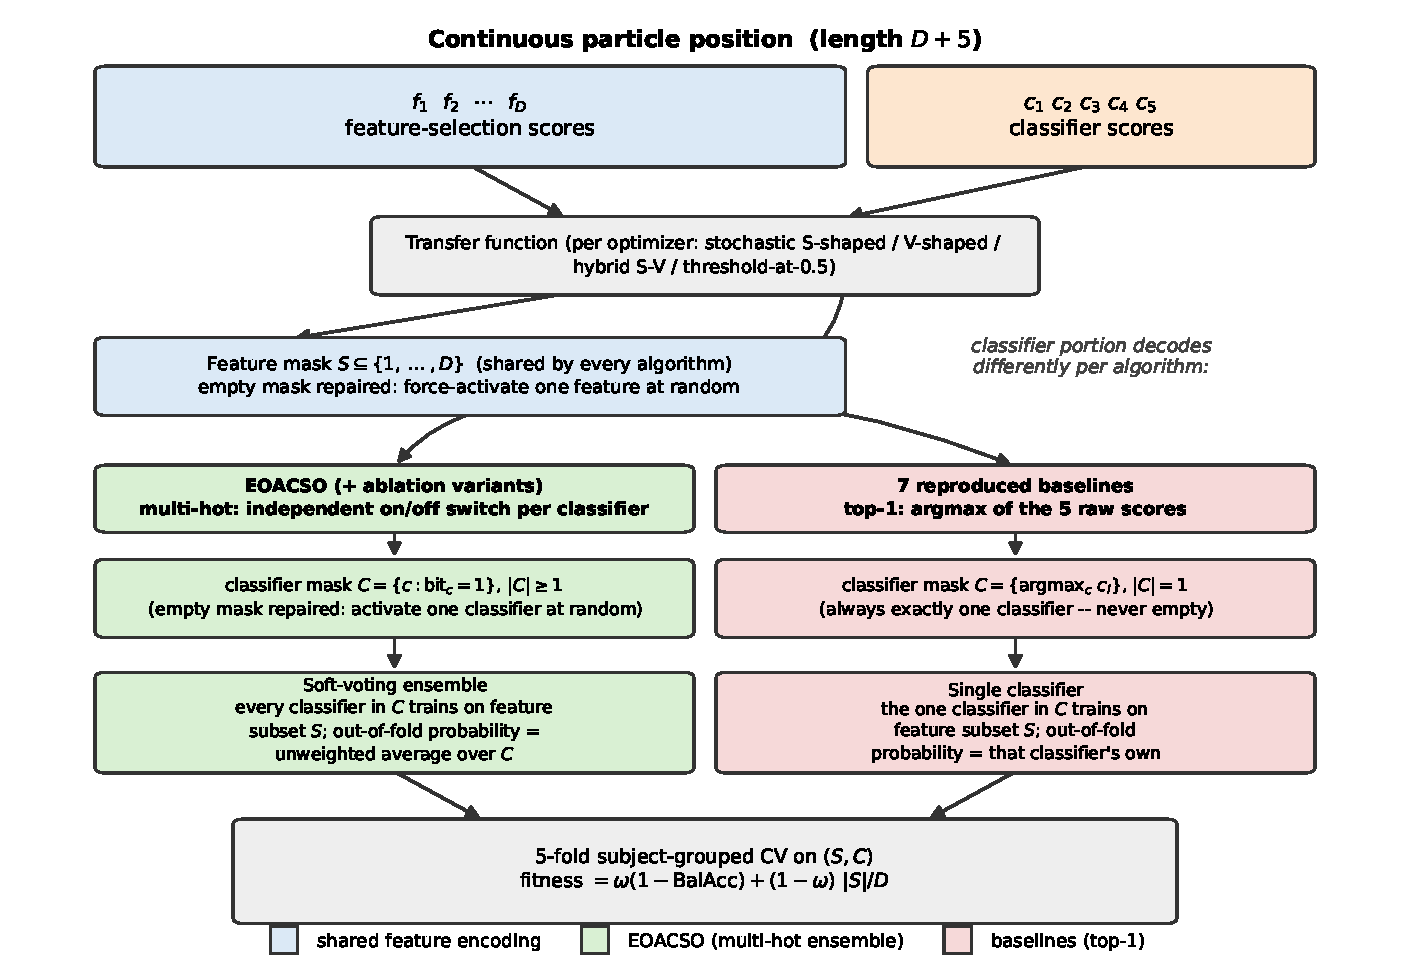
\includegraphics[width=\linewidth]{figures/encoding_diagram.pdf}
  \caption{Encoding and decoding schematic. A continuous particle
    position of length $D+5$ splits into a shared feature-score segment
    and a 5-dimensional classifier-score segment. Both pass through the
    optimizer's transfer function; the resulting feature mask $S$ is
    shared by every algorithm, while the classifier mask $C$ is decoded
    multi-hot for EOACSO (an equal-weight soft-voting ensemble over
    however many classifiers are switched on) and top-1 for the 7
    reproduced baselines (exactly one classifier, via argmax). Both
    branches feed the same 5-fold subject-grouped cross-validation and
    fitness function (Section~\ref{sec:3.4}).}
  \label{fig:encoding}
\end{figure}

Figure~\ref{fig:encoding} summarizes this decoding scheme end to end.

Every algorithm in this study binarizes its continuous position through
one of four transfer functions (Figure~\ref{fig:transfer}). EOACSO uses
the classic stochastic S-shaped transfer function: bit $=1$ with
probability $\sigma(x)$, the logistic sigmoid, so probability of
selection increases monotonically with $x$. BGWO, HybridGWO, and QMFO
also use this same curve, since their source papers do not specify a
transfer function. BPSO, BBOA, and BWOA instead use the hybrid
S-shaped/V-shaped scheme of Hashemi et al.\ (Eq.\ 8): each generation, both
an S-shaped candidate bit-vector and a V-shaped candidate bit-vector are
generated, both are evaluated, and whichever scores better fitness is
kept -- this is a selection rule between two binarizations, not a fifth
curve. Their S-shaped curve, notably, decodes in the \emph{opposite}
direction from EOACSO's: bit $=1$ with probability $1-\sigma(x)$, per that
paper's own literal equation (Eq.\ 4--5), so this is a documented,
intentional fidelity choice rather than an inconsistency in this
project's own code. Their V-shaped curve (Eq.\ 6--7) instead governs
whether the \emph{previous} bit flips, with flip probability peaking at
$x=0$ and decaying as $|x|$ grows. Finally, MGWO-eP and mHGS work
natively in $[0,1]$ (per their own papers' convention) and binarize with
a simple hard threshold at 0.5, with no stochastic component.

\begin{figure}[t]
  \centering
  
\includegraphics[width=\linewidth]{figures/transfer_functions.pdf}
  \caption{The four transfer functions used in this study. Each closed
    form was derived directly from the actual implementation
    (\texttt{src/optimizers/base.py}, \texttt{src/optimizers/transfer.py})
    and cross-checked by Monte Carlo simulation of the real code before
    plotting, so the curves shown cannot drift out of sync with it.
    Top-left: EOACSO's stochastic S-shaped curve. Top-right: the
    baselines' S-shaped curve, decoding in the opposite direction per
    Hashemi et al.'s literal equation. Bottom-left: the baselines'
    V-shaped curve, governing the probability of flipping the previous
    bit. Bottom-right: the hard threshold used natively in $[0,1]$ by
    MGWO-eP and mHGS.}
  \label{fig:transfer}
\end{figure}

\subsection{Fitness Function}
\label{sec:3.4}

Every candidate solution is scored by a single scalar fitness, combining
diagnostic performance with a feature-parsimony penalty:
\begin{equation}
  \text{fitness} = \omega \cdot (1 - \text{BalAcc}) + (1 - \omega) \cdot \frac{|S|}{D},
  \label{eq:fitness}
\end{equation}
where $\text{BalAcc}$ is the out-of-fold balanced accuracy (the average of
sensitivity and specificity, robust to Oxford's class imbalance
\cite{Brodersen:2010}) achieved by the decoded feature subset and
classifier (or ensemble of classifiers,
for EOACSO), $|S|$ is the number of selected features, $D$ is the total
number of available features, and $\omega = 0.9$ weights diagnostic
performance nine times as heavily as feature count. This value was chosen
so that a modest reduction in feature count is rewarded only when it does
not come at a material cost to balanced accuracy -- reflecting the
clinical framing of this study as favoring parsimonious acoustic
measurement panels for low-burden screening (Section~\ref{sec:2.1}),
without allowing the parsimony term to dominate the primary diagnostic
objective. Lower fitness is better; every optimizer in this study is
implemented as a minimizer.

\subsection{EOACSO: Elite-guided Opposition-based Archive Competitive Swarm Optimizer}
\label{sec:3.5}

EOACSO extends the original Competitive Swarm Optimizer (CSO)
\cite{Cheng:2015} with three strategies, each independently toggleable to
support the ablation study (Section~\ref{sec:3.6}).

\textbf{Base algorithm (CSO).} Each generation, the population of $N$
particles (an even number) is randomly paired into $N/2$ one-on-one
competitions. Within each pair, the fitter particle (the \emph{winner})
passes to the next generation completely unchanged; the weaker particle
(the \emph{loser}) updates its velocity and position toward the winner:
\begin{align}
  v_l &\leftarrow r_1 v_l + r_2 (x_w - x_l) + \phi \, r_3 (\bar{x} - x_l), \\
  x_l &\leftarrow x_l + v_l,
\end{align}
where $x_w, x_l$ are the winner's and loser's positions, $\bar{x}$ is the
population mean position, $r_1, r_2, r_3$ are independent uniform random
vectors, and $\phi$ is CSO's social-term control coefficient (Eq.\ 25--26,
\cite{Cheng:2015}), which is exactly 0 for the swarm sizes used in this
study ($N=30 \le 100$) -- so plain CSO at this scale has no mean-position
pull at all, only the winner-attraction and inertia terms.

\textbf{Strategy 1 -- Elite-guided update (\texttt{enable\_elite\_guided}).}
Replaces CSO's uninformative $\phi\,r_3(\bar{x}-x_l)$ mean-position term
with a pull toward an elite solution sampled uniformly at random from the
diversity archive (Strategy 3 below):
\begin{equation}
  v_l \leftarrow r_1 v_l + r_2 (x_w - x_l) + \lambda(t) \, r_3 (x_{\text{elite}} - x_l),
\end{equation}
where $\lambda(t)$ grows linearly from 0.1 to 0.9 over the run, so early
generations weight the elite-guidance term lightly (favoring
exploration) while late generations weight it heavily (favoring
exploitation around good solutions already found). If the archive is
empty, $x_{\text{elite}}$ falls back to the global best position found so
far.

\textbf{Strategy 2 -- Stagnation-triggered Opposition-Based Learning
(\texttt{enable\_obl}).} If the global best fitness has not improved for
\texttt{stagnation\_limit} (default 5) consecutive generations, the worst
\texttt{reinit\_fraction} (default 30\%) of the population, ranked by
fitness, is reinitialized to its opposite point in the search space,
$x' = lb + ub - x$ (with $lb=-ub$ under this study's symmetric position
bounds), and re-evaluated. This is a standard opposition-based learning
mechanism \cite{Tizhoosh:2005} for escaping local optima: if the current
region of the search space has stagnated, the diametrically opposite
region is sampled directly rather than relying on gradual
velocity-driven drift to reach it.

\textbf{Strategy 3 -- Diversity-preserving elite archive
(\texttt{enable\_archive}).} A bounded external archive (default capacity
30) maintains a Pareto-non-dominated set of solutions on two objectives:
error rate ($1-\text{BalAcc}$) and feature ratio ($|S|/D$). A new solution
is inserted only if no existing archive member dominates it on both
objectives simultaneously; any archive members it dominates are removed.
When the archive exceeds capacity, the member with the smallest Hamming
distance to its nearest neighbor (over the concatenated feature and
classifier masks) is removed, preserving the most mutually diverse subset
of non-dominated solutions rather than simply the most recently added.
The archive serves two purposes: during the search, it supplies the elite
samples consumed by Strategy 1; after the search, its final contents are
themselves a set of alternative accuracy/parsimony trade-off solutions
(Section~\ref{sec:5.5}), not only the single best solution returned.

Turning all three strategies off reproduces plain CSO on this study's own
joint feature-and-classifier encoding (denoted \texttt{CSO\_vanilla} in
the ablation study), rather than the original CSO's feature-selection-only
formulation.

\subsection{Comparison Methods and Ablation Design}
\label{sec:3.6}

\textbf{Reproduced literature baselines.} Seven metaheuristic
feature-selection methods from five recent source papers are
re-implemented from their published equations and evaluated under this
study's own encoding, fitness function, and cross-validation protocol
(not each source paper's own classifier or data split), enabling a
controlled, like-for-like comparison against EOACSO: BPSO and BBOA
(binary particle swarm and butterfly optimization, hybrid S-shaped/
V-shaped transfer function) \cite{Hashemi:2026}; BGWO and HybridGWO
(binary grey wolf optimizer, and a whale-optimization-then-grey-wolf
refinement cascade) \cite{AlNajjar:2024}; MGWO-eP (grey wolf optimizer
with an exponentially-decaying exploration coefficient)
\cite{Santhosh:2025}; mHGS (modified Hunger Games Search with a
mean-of-best-4 local escaping operator) \cite{Hashim:2023}; and QMFO
(Mayfly Algorithm with a quantum-rotation-gate mutation operator)
\cite{Mansour:2024}. A third variant originally reproduced from Hashemi
et al. \cite{Hashemi:2026}, BWOA (binary whale optimization), was also
implemented but is excluded from the reported comparison: of the 8
originally reproduced baselines, its results were consistently the
weakest and least consistent with its own source paper's claims, so it is
not included as a fair comparison point (see Section~\ref{sec:6.4} for
further discussion). Where a source paper does not fully specify an
equation
(most application papers cite only the base metaheuristic by name), the
canonical published form of that equation is used instead, and every such
gap-fill is documented in the corresponding source file's docstring for
transparency.

\textbf{Ablation variants.} Five variants isolate EOACSO's three
strategies subtractively, starting from the full method and removing one
strategy at a time down to plain CSO: \texttt{EOACSO\_full} (all three
enabled), \texttt{EOACSO\_no\_elite\_guided}, \texttt{EOACSO\_no\_obl},
\texttt{EOACSO\_no\_archive} (each with exactly one strategy disabled),
and \texttt{CSO\_vanilla} (all three disabled).

\textbf{Equal evaluation budget.} Every optimizer -- EOACSO variants and
baselines alike -- is compared under an equal fitness-evaluation budget
(\texttt{max\_evaluations}), not equal generation count, since different
algorithms spend different numbers of fitness evaluations per generation
(e.g., the hybrid S-shaped/V-shaped transfer function used by
BPSO/BBOA evaluates two binarization candidates per individual per
generation; mHGS's production and escaping operators each conditionally
add extra evaluations). A population size of 30 and an evaluation budget
of 3000 fitness evaluations per run are used throughout; each algorithm's
internal time-dependent schedule (e.g. EOACSO's $\lambda(t)$, the grey
wolf family's exploration coefficient) is normalized against a
\emph{nominal} generation count derived from this budget, while the
budget itself remains the sole stopping condition.

\textbf{Independent runs and seeding.} Each algorithm-dataset combination
is run for multiple independent seeds (seed $= 2026 + 50 \times$
run index, so seeds do not overlap across runs), with all stochastic
elements -- population initialization, transfer-function sampling, and
the cross-validation fold assignment for that seed -- freshly drawn each
run. The ablation study reported in this manuscript uses 5 independent
runs per variant per dataset; the head-to-head comparison against the 7
baselines uses a larger number of runs to support the statistical testing
described in Section~\ref{sec:3.8}.

\subsection{Evaluation Metrics}
\label{sec:3.7}

For every run, the out-of-fold predictions used to compute fitness
(Section~\ref{sec:3.4}) are also used to report a full panel
of standard diagnostic-performance metrics, computed once per run (not
re-derived from the fitness value): accuracy, balanced accuracy,
\textbf{sensitivity (recall)}, \textbf{specificity}, precision, F1-score,
and area under the receiver operating characteristic curve (ROC-AUC).
Sensitivity and specificity are reported alongside the more
ML-conventional accuracy/F1/AUC metrics because they are the standard
vocabulary for evaluating a clinical screening tool: sensitivity
quantifies the fraction of true PD cases the pipeline would flag (missed
cases have direct clinical cost), while specificity quantifies the
fraction of healthy individuals correctly spared unnecessary follow-up.
Feature-selection ratio ($|S|/D$) and the identity of the selected
feature subset and active classifier(s) are also recorded for every run,
supporting the feature-interpretability analysis in
Section~\ref{sec:5.5} and the classifier-preference analysis in
Section~\ref{sec:5.6}.

\subsection{Statistical Analysis}
\label{sec:3.8}

Because every algorithm is run under the same set of seeds (and therefore
the same sequence of cross-validation fold assignments per run index),
per-run performance scores across algorithms are paired rather than
independent samples. The Wilcoxon signed-rank test \cite{Wilcoxon:1945} is
used for pairwise comparisons between EOACSO and each individual baseline
or ablation variant, and the Friedman test \cite{Friedman:1937} is used
to test for an overall difference across the full set of compared
algorithms before conducting pairwise follow-up tests, guarding against
inflated false-positive rates from running many uncorrected pairwise
tests -- following established recommendations for comparing multiple
classifiers across multiple datasets \cite{Demsar:2006}
(\texttt{src/experiments/stats.py}).

\subsection{Implementation Details}
\label{sec:3.9}

All optimizers, the fitness evaluator, and the experiment orchestration
are implemented in Python (NumPy for optimizer internals; scikit-learn
\cite{Pedregosa:2011} and XGBoost \cite{Chen:2016} for the candidate
classifiers). Runs are executed serially
(one fitness evaluation, and one classifier fit, at a time) on
consumer-grade hardware; each completed run is checkpointed to disk
immediately so that a long-running batch of independent runs can be
resumed from the last completed run rather than restarted from scratch
after an interruption.
